%************************************************
\chapter{Particle Detection with Liquid Xenon}

\label{ch:LXeTPCs} 
%************************************************

Liquid xenon detectors are powerful tools for rare event searches. In particular, the dual phase \ac{LXe} \ac{TPC} has been very successful in accessing \ac{WIMP} parameter space and currently holds the worlds most sensitive limits on \ac{WIMP}s. This chapter covers particle interactions in liquid xenon and explains the operating principles of \ac{LXe} \ac{TPC}s. The features of these detectors that make them especially useful for \ac{WIMP} searches are discussed, and some methods by which their function can be adapted to search for other dark matter candidates are given.

\section{Liquid Xenon as a Detector Medium}
 This section first describes the properties of \ac{LXe} and the microphysics of signal generation in xenon. A few examples of xenon detector programs are given, and the basic principles of \ac{TPC}s are described.

\subsection{Properties of Liquid Xenon}
Liquid xenon has many properties relevant to particle detection, particle identification, and also many properties related to the ease of detector operation:

\begin{itemize}

\item The density of \ac{LXe} is 2.9~g/cm$^{3}$ at 170~K, which is higher than other noble elements (\ac{LAr} has density 1.4~g/cm$^{3}$ at 87~K). The advantage in this two-fold: (1) large target mass gives a large exposure, increasing the sensitivity of the dark matter search; (2) self-shielding: high density targets are capable of stopping external radiation, producing an ultra-low-background volume in the center of the detector where rare-event searches can be performed (this region is called the ``fiducial volume'').
  
\item Xenon gas is easily liquefied with liquid nitrogen (77~K) or commercially available pulse tube refrigerators.

\item Xenon has no long-lived radioisotopes that cause troublesome backgrounds. The two exceptions are the 2$\nu\beta\beta$ decays of $^{136}$Xe (natural abundance 8.875\%) with measured half-life of $T_{1/2}^{0\nu\beta\beta} = 2.1 \times 10^{21}$~years and $^{134}$Xe (natural abundance 10.4\%) with half-life $T_{1/2}^{0\nu\beta\beta} > 8.7 \times 10^{20}$~years. The long half-life and relatively low abundance together result in a very low count rate, and the isotopes can be used to search for neutrino-less double beta decay ($0\nu\beta\beta$).
  
\item Particles interacting in \ac{LXe} create excitons and electron ion-pairs, producing detectable quanta: scintillation photons and ionization electrons, respectively (described in Section~\ref{sec:signal_generation}).
  
\item Xenon is transparent to its own scintillation light (described in Section~\ref{sec:signal_generation}). The scintillation light is of wavelength $\lambda$~=~178~nm and can be directly detected with current \ac{PMT} technology, and doesn't require the use of e.g wavelength shifter. 

\item Xenon has high light and charge yields, and therefore a low threshold for producing detectable quanta. A useful quantity is the so-called ``W-value'' of \ac{LXe}: W = 13.7 $\pm$ 0.2 eV \cite{Dahl2009}. The W-value, analogous to a work-function, is a measure of the average energy expenditure to produce one quanta (scintillation photon or an ionization electron) from liquid xenon. 

\item Ionization electrons produced in particle interactions can be drifted away from the interaction site and detected independently of the scintillation signal. This is the basic principle of \ac{TPC}s, which provides measurement of both light and charge (see Section~\ref{sec:xe_detectors}).  
% extracted into a gaseous region via applied electric fields, where they undergo proportional scintillation. By this method, a single electron is amplified many-fold into detectable photons. This is the basic operating principle of dual-phase \ac{TPC}s, which makes even a single ionization electron detectable. Single-phase \ac{TPC}s can also 
    
\item Xenon, as a noble element, is easily purified with a heated getter to rid electronegative impurities. Some of these impurities absorb xenon scintillation light, e.g. N$_{2}$, and others can absorb electrons, interfering with the ionization signal in \ac{TPC}s, e.g. O$_{2}$.

\item \ac{LXe} \ac{TPC}s are easily scalable: creating a large homogenous volume is straightforward. In contrast, solid state detectors, such as cryogenic Ge, are more difficult to scale up directly and require instead the production of multiple small modules (O(10)~cm) which each must be instrumented separately.  
  
\item The comparatively large mass of xenon allows it to be purified of other noble gasses via gas chromatography \cite{LUXKrRemoval2018} and cryogenic distillation \cite{Xe1TKrRemoval2017}. As other noble gasses cannot be removed via getter, this feature is extremely useful in removing the troublesome background of $^{85}$Kr decay. $^{85}$Kr decays via beta emission to stable $^{85}$Rb with a half-life of 10.8 years and Q$_{\beta}$ = 687~keV. The decay proceeds directly to the $^{85}$Rb ground state with a branching ratio of 99.6\%. Since no de-excitation of $^{85}$Rb follows, this beta decay cannot be rejected as background by coincidence with a gamma, and relies purely on the ability to discriminate between \ac{WIMP}-like \ac{NR} and beta- or gamma- produced \ac{ER}. While ER/NR discrimination is one of the features of \ac{LXe} \ac{TPC}s (described further in Section~\ref{sec:er_nr_discrimination}), leakage of \ac{ER} events in to the \ac{NR} signal region can occur and the best mitigation is to remove as much of the $^{85}$Kr as possible. Single-phase \ac{LXe} detectors, with no ER/NR discrimination, benefit greatly from the ability to remove $^{85}$Kr.
   
\end{itemize}


\subsection{Scintillation and Ionization Signal Generation}
\label{sec:signal_generation}
Signal generation in xenon is summarized in Figure~\ref{fig:sig_gen}. A particle can interact with a xenon atom through interaction with an orbiting electron, creating an \ac{ER}, or though an interaction with the xenon nucleus \ac{NR}, where the nucleus is imparted with momentum and recoils. The recoiling electron or nucleus loses energy via interaction with neighboring xenon atoms, creating more excited atoms and electron-ion pairs. The excited xenon atoms, Xe$^{*}$, combine with other atoms to form an excited dimer (also called excitons or excimers), Xe$_{2}^{*}$. The excited dimer forms two states: a triplet and a singlet, which de-excite with the emission of a 178~nm photon. The lifetimes of the triplet and singlet are measured to be 24~ns and 3~ns, respectively \cite{Mock2014}. Since the scintillation light is produced by the excimer, which has a different electronic structure than atomic xenon, the light is free to propagate through the detector and will not be absorbed by the atomic xenon. The Xe$^{+}$ ions of the electron-ion pairs combine with other Xe atoms to form dimers Xe$_{2}^{+}$, and these dimers can combine with electrons (from the electron-ion pairs) to form excitons, Xe$_{2}^{*}$, which then decay and produce additional 178~nm scintillation photons. This process is called recombination. If no electric field is applied, all electron-ion pairs recombine to produce additional scintillation photons. If an external electric field is present, some electrons can be drifted away from the interaction site to be detected with other methods. 

\begin{figure}[htbp]
\begin{center}
%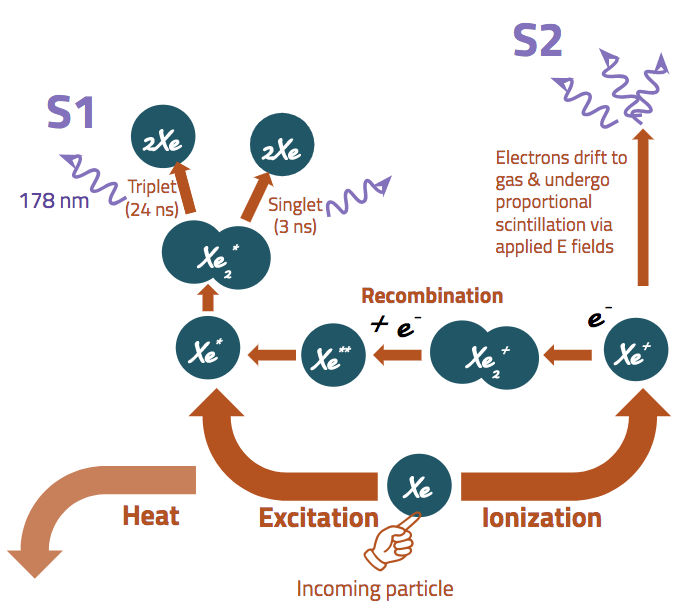
\includegraphics[width=\textwidth]{figures/lxetpcs/signal_generation_in_lxe_tpcs.png}
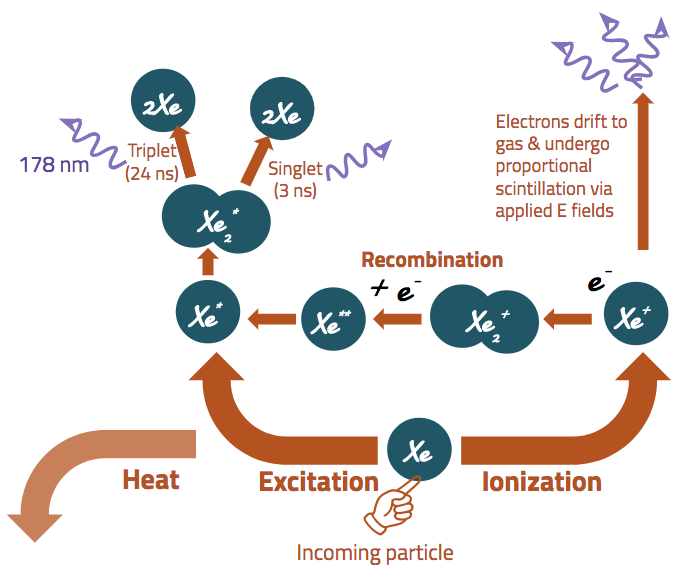
\includegraphics[width=\textwidth]{figures/lxetpcs/signal_generation_in_lxe.png}
\caption{ Diagram summarizing the generation of the scintillation and ionization signal generation in dual-phase xenon time projection chambers.}
\label{fig:sig_gen}
\end{center}
\end{figure}

 
\FloatBarrier
\section{Types of Xe Detectors}
\label{sec:xe_detectors}
There are a variety of detectors that use xenon as their target material. Xenon is utilized in single phase detectors which can be comprised of liquid or gas. Xenon is also utilized in dual-phase detectors which have both liquid and gas regions. This section gives examples of a few types of Xe detector programs, commenting on the challenges that affect their sensitivities. 

\subsection{XMASS: A Single Phase LXe Detector}
XMASS is a single phase liquid xenon detector shown in Figure~\ref{fig:xmass}; it measures a scintillation-only signal \cite{Abe2013}. There is no electric field, so all electron-ion pairs created in a particle interaction recombine to emit scintillation photons. XMASS is a multipurpose experiment, which aims to study solar neutrinos, double beta decay, and \ac{WIMP}s \cite{Chepel2013}.

\begin{figure}[htbp]
\begin{center}
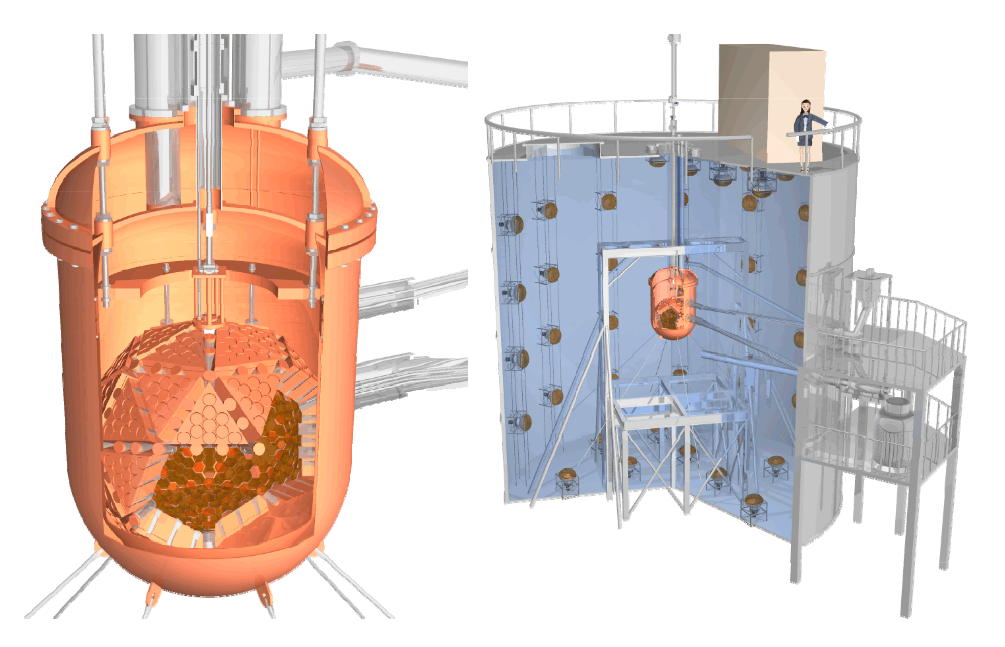
\includegraphics[width=\textwidth]{figures/lxetpcs/xmass.png}
\caption{Diagram of the XMASS detector and water tank. Figure from \cite{Chepel2013}. }
\label{fig:xmass}
\end{center}
\end{figure}

The sensitivity of liquid xenon detectors to low energy recoils depends on their ability to detect the 178~nm scintillation photons with high-efficiency. High \ac{QE} \ac{PMT}s constructed with ultra-low radioactivity materials are the go-to instrument for this purpose. In addition to high-efficiency photon-detectors, liquid xenon detectors must also have high geometrical light collection efficiency to optimize sensitivity. Single-phase liquid xenon detectors such as XMASS aim to maximize light-collection by with a spherical geometry, endeavoring to cover 4$\pi$ steradians surrounding the \ac{LXe}. The XMASS detector geometry accomplishes photocathode coverage of \~62\%. Two types of Hamamatsu \ac{PMT}s are used (R10789-11 and R10789-11MOD), which have \ac{QE} of 28\%. Putting this together, XMASS quotes a final signal collection efficiency of 20\% \cite{Abe2013}, \cite{XMASSCollaboration2018}. 

%Dual-phase \ac{TPC} detectors are lined with \ac{PTFE} to take advantage of its extremely high (~99\%) reflectivity for 178~nm light in \ac{LXe} \cite{Neves2017}. The \ac{LUX} detector uses a cylindrical geometry, with all non-light-collectiing surfaces lined with \ac{PTFE}, and Hamamatsu R8778 \ac{PMT}s (\ac{QE} of 33\%) only on the top and bottom of the detector (low photocathode coverage), to accomplish a light collection efficiency of 90\% \cite{Faham2014a}.
\FloatBarrier
\subsection{EXO-200: A Single Phase LXe TPC}
The EXO-200 experiment is a single phase liquid xenon \ac{TPC} shown in Figure~\ref{fig:exo200}. \ac{TPC}s detect the scintillation photons and ionization electrons separately. The scintillation photons are detected promptly, while the ionization electrons are drifted away from the interaction site to be detected elsewhere. EXO-200 uses avalanche photodiodes to collect the scintillation photons and crossed-wire planes to collect the ionization electrons \cite{Auger2012}. 

\begin{figure}[htbp]
\begin{center}
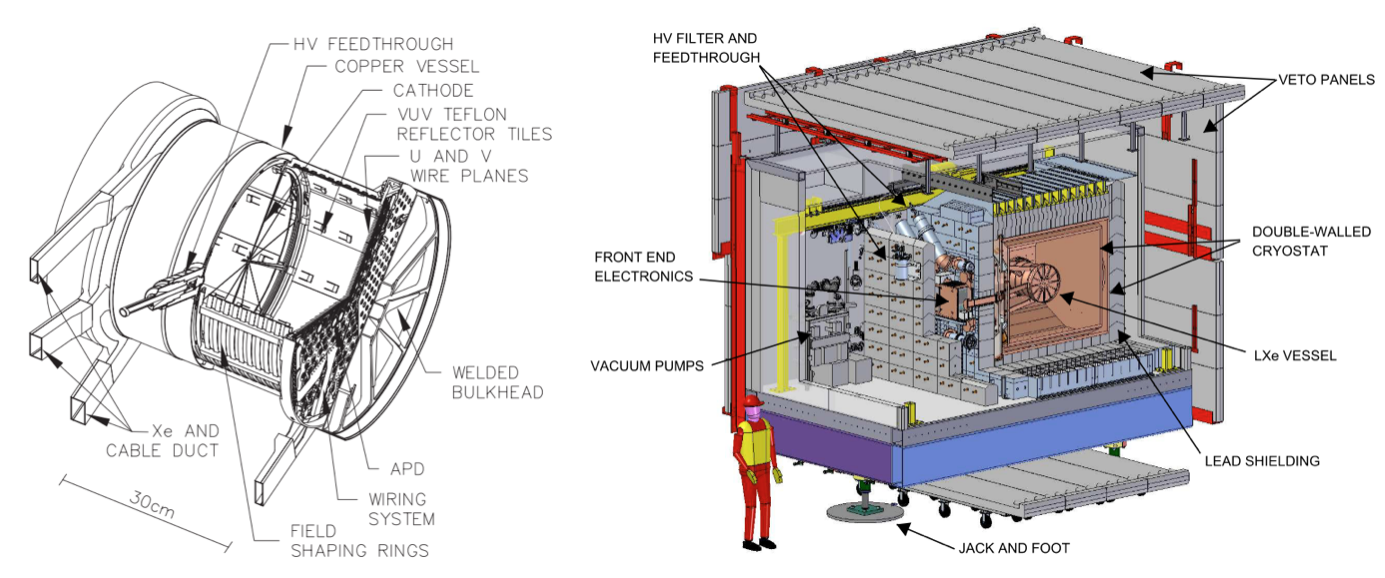
\includegraphics[width=\textwidth]{figures/lxetpcs/exo200.png}
\caption{Diagram of the EXO-200 detector and systems. Figure from \cite{Auger2012}. }
\label{fig:exo200}
\end{center}
\end{figure}

In addition to light-collection efficiency, the sensitivity of \ac{TPC} xenon detectors also depends on their ability to collect signal from the ionization electrons. There are challenges in delivering \ac{HV} to liquid xenon in order to set up the electric field which drifts the ionization electrons (some of these challenges are illustrated in Chapter \ref{ch:testbed}). Additionally, electronegative impurities such as oxygen (O$_{2}$) present in the detector attract and capture ionization electrons as they drift, eating away the ionization signal. These non-noble impurities are removed by constantly circulating the xenon through a heated zirconium getter and returning it to the detection volume. Purification through a getter must be done in gaseous phase, so liquid xenon removed from the detection volume is evaporated, passed through the getter via a circulation system, and re-condensed into the detection volume. 

%\ac{LUX} is a dual-phase xenon \ac{TPC}, where ionization electrons produced in the large liquid region are drifted and extracted into gaseous xenon via applied electric fields, where they undergo proportional scintillation. The proportional scintillation light is the same 178~nm wavelength as scintillation in the liquid produced in the liquid, and it is similarly collected via high \ac{QE} \ac{PMT}s.
\FloatBarrier
\subsection{LUX: A Dual Phase LXe TPC}
The \ac{LUX} experiment is a dual phase \ac{LXe} \ac{TPC} shown diagrammatically in Figure~\ref{fig:tpc}; much more detail about the \ac{LUX} detector and components can be found in Chapter~\ref{ch:lux}. A dual phase liquid xenon \ac{TPC} is a type of \ac{TPC} with a large liquid target volume and a small region of xenon vapor above the liquid volume, instrumented with light sensors (typically \ac{PMT}s). \ac{LUX} uses high \ac{QE} \ac{PMT}s (Hamamatsu R8778) to detect the prompt scintillation photons; this primary signal is called S1. The ionization electrons are drifted upward to the gas region by an applied electric field, and extracted across the liquid-gas boundary by a higher electric field, where they undergo proportional scintillation and produce a second signal called S2, which is also detected by the \ac{PMT}s. 

\begin{figure}[htbp]
\begin{center}
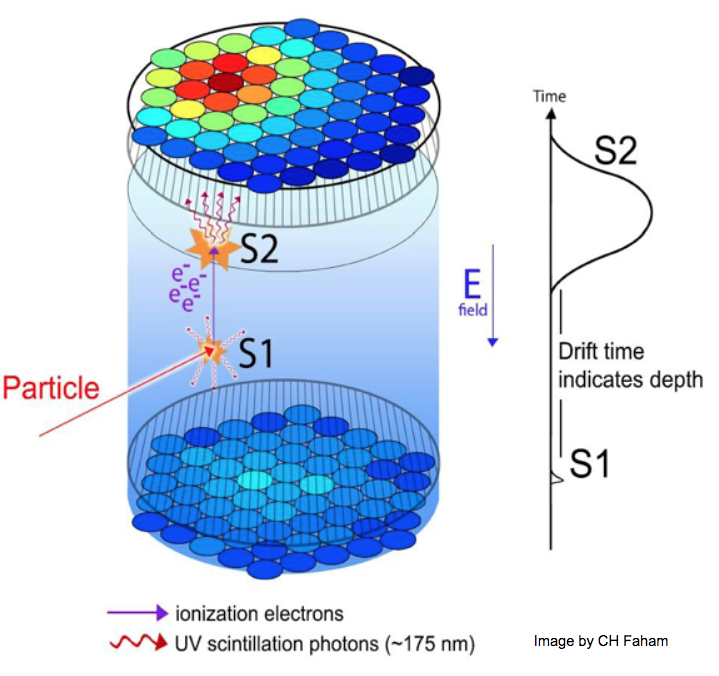
\includegraphics[width=\textwidth]{figures/lxetpcs/TPC.png}
\caption{ Diagram of a dual-phase xenon time projection chamber. The time difference between S1 and S2 gives the depth ($z$) of the interaction, and $(x,y)$ is reconstructed from the S2 signal.}
\label{fig:tpc}
\end{center}
\end{figure}

The electric fields are supplied by a series of electrodes, composed of wire planes, grids, or chemically etched meshes, held at constant voltages. The bottom-most field-producing electrode is called the cathode. At the top of the liquid region is the gate or extraction electrode, followed O(1)~cm by the anode in the gas. The liquid region is often referred to as the ``drift region'' and region between the gate and anode is referred to as the ``extraction region''. The electrons are extracted from liquid to gas with some efficiency, called the \ac{EEE}. In addition to the challenges of light-collection, \ac{HV} delivery, and xenon purification, \ac{EEE} plays an important role in the operation of dual phase \ac{LXe} \ac{TPC}s, and is discussed further in Chapter~\ref{ch:etrains}.
%A particle interacting in a noble liquid or gas target deposits energy into scintillation and ionization channels (Section \ref{sec:signal_generation}). The basic operating principle of \ac{TPC}s is to drift the ionization electrons away from the interaction site and detect them at a later time than the scintillation signal is detected. A dual phase liquid xenon \ac{TPC} is a type of \ac{TPC} with a large liquid target volume and a small region of xenon vapor above the liquid volume, instrumented with light sensors (typically \ac{PMT}s). 

\ac{LUX} is lined with \ac{PTFE} to take advantage of its extremely high ($\sim$99\%) reflectivity for 178~nm light in \ac{LXe} \cite{Neves2017}. The \ac{LUX} detector uses a cylindrical geometry, with all non-light-collecting surfaces lined with \ac{PTFE}. The Hamamatsu R8778 \ac{PMT}s (\ac{QE} of 33\%) are installed only on the top and bottom of the detector, but the reflective \ac{PTFE} allows \ac{LUX} to accomplish an S1 light collection efficiency of 11\% \cite{LUX:Run03Comprehensive}.

The S2 in a dual phase \ac{TPC} plays two important roles: (i) internal amplification of the signal, whereby a few electrons are transformed into O(10) times as many photons (ii) $(x,y)$ localization via \ac{PMT} hit pattern. The time spacing of the S1 and S2 signals (called ``drift time'') can be converted to depth ($z$) of the interaction, providing full $(x,y,z)$-reconstruction of the interaction position. The full position reconstruction capability allows \ac{LXe} \ac{TPC}s to select a fiducial volume in the center of the detector that has ultra low background, as the xenon medium self-shields from radioactive backgrounds located in and on detector components. 

The remainder of this chapter focuses on the \ac{LXe} \ac{TPC} technology for dark matter detection. 

\FloatBarrier
\section{Energy Reconstruction in Dual Phase LXeTPCs}
\label{sec:energy_reconstruction}
Energy reconstruction in dual phase xenon \ac{TPC}s comes from the measurable quantities, S1 and S2, but begins with the number of excitons $n_{ex}$  and electron-ions pairs $n_{i}$ generated at the interaction site. 
\begin{equation}
E = f W (n_{ex} + n_{i} )
\end{equation}

where $E$ is the deposited energy. $W$ is the average energy needed to produce a single excited or ionized atom, $W = 13.7 \pm 0.2$~eV \cite{Mock2014}. The quenching factor, $f$, is 1 for electronic recoils but $f \neq 1$ for nuclear recoils. For now, take the case of electronic recoils and set $f=1$. This equation can be rewritten:

\begin{equation}
E_{ER} = W \Big(1 + \frac{n_{ex}}{n_{i}} \Big) n_{i}
\end{equation}

The ratio of excitons to ions is constant for electron recoils $n_{ex}/{n_{i}} = 0.2$ \cite{LUX:YieldsAndRecombination}. As discussed in Section \ref{sec:signal_generation}, each exciton deexcites, emitting a 178~nm photon, some fraction $r$ of the initial electron-ion pairs recombine and form additional excitons. The total number of prompt scintillation photons created by the interaction is then:

\begin{equation}
n_{\gamma} = \Big(r + \frac{n_{ex}}{n_{i}} \Big) n_{i}
\end{equation}

And the total number of electrons escaping recombination is:

\begin{equation}
n_{e} = (1 - r ) n_{i}
\end{equation}

Thus, the effect of recombination is to ``trade-out'' electrons for photons, but the total number of quanta is conserved (Figure~\ref{fig:recombination} (left)). The amount of recombination depends on applied electric field, \ac{LXe} density, and particle energy \cite{LUX:YieldsAndRecombination}. In the case of the 122~keV electron recoils in Figure~\ref{fig:recombination} (right): at low fields, most of the electron-ion pairs recombine, which results in more scintillation photons. As the applied electric field increases, more electrons are pulled away from the interaction site resulting in fewer scintillation photons and more ionization electrons. These amounts of photons and electrons are referred to as the scintillation and ionization yields. The two quantities, $n_{\gamma}$  and $n_{e}$ relate directly to the observable S1 and S2 signals, so we can rewrite Equation~\ref{eq:energy} as follows:

\begin{equation}
\label{eq:energy}
\begin{split}
E_{ER} &= W (n_{\gamma} + n_{e} ) \\
   &= W \Big(\frac{S1}{g_{1}} + \frac{S2}{g_{2}} \Big)
\end{split}
\end{equation}

S1 and S2 are in units of detected photons (phd) or photoelectrons (phe), and $g_{1}$ and $g_{2}$ are detector gains in units of phd/quanta or phe/quanta\footnote{An distinction should be made between the traditional units of phe and the units of phd which are used in many LUX publications. The Hamamatsu R8778 PMTs used in LUX emit two photoelectrons for a single VUV photon $\sim$20\% of the time \cite{Faham2015}, but the PMT gain calibration photons (from blue LEDs) do not. LUX performed additional calibration with VUV photons to account for the difference, and report detected photons instead of photoelectrons \cite{LUX:Run03Comprehensive}}. $g_{1}$ is the detection efficiency for the prompt scintillation photons: it is a product of the average geometrical light collection efficiency and the average \ac{PMT} \ac{QE}. Typical values for $g_{1}$ are in the range of 0.1-0.2. $g_{2}$ is the analogous quantity for S2 proportional scintillation light: it is a product of the \ac{EEE} and the average number of detected photons produced by one extracted electron. Typical values for $g_{2}$ are in the range 10-60.



\begin{figure}[htbp]
\begin{center}
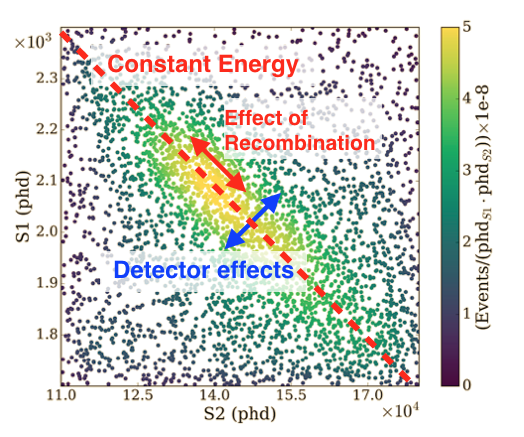
\includegraphics[width=\halffig]{figures/lxetpcs/recombination.png}
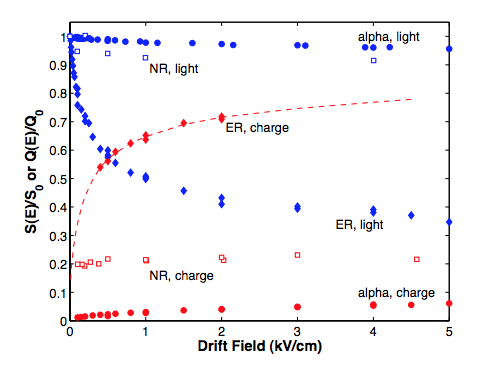
\includegraphics[width=\halffig]{figures/lxetpcs/yields.png}
\caption{(left) Plot illustrating the effect of recombination and detector effects on a line source (127Xe), courtesy of E. Pease. (right) Field dependence of scintillation and ionization yield in LXe for 122 keV electron recoils (ER), 56.5 keVr nuclear recoils (NR) and 5.5 MeV alphas, relative to the yield with no drift field from \cite{Aprile2010}.}
\label{fig:recombination}
\end{center}
\end{figure}

To properly reconstruct the energy of nuclear recoils, we must revisit the quenching factor factor $f$. Equation~\ref{eq:energy} then becomes:

 \begin{equation}
 \begin{split}
E_{NR} &= f W (n_{\gamma} + n_{e} ) \\
   &= f W \Big(\frac{S1}{g_{1}} + \frac{S2}{g_{2}}\Big)
 \end{split}
\end{equation}

This equation can be rewritten:

 \begin{equation}
 \label{eq:combined_energy}
E_{NR} = f E_{ER} = \frac{E_{ER}}{\mathcal{L}}
\end{equation}

where $\mathcal{L}$ is Lindhard's factor. Lindhard's factor accounts for the fraction of energy lost to atomic motion (heat) in nuclear recoils \cite{Lindhard1963}. Recall that a recoiling Xe nucleus loses energy in interactions with neighboring Xe atoms to produce S1 and S2; it is the energy partitioning in this cascade with neighboring atoms that results in different energy scales for \ac{ER} and \ac{NR}. Lindhard showed that the energy partitioned in nuclear interactions and electron interactions (as opposed to heat) from a recoiling xenon nucleus is:

 \begin{equation}
 \label{eq:lindhard}
\mathcal{L} = \frac{k g(\epsilon)}{1 + k g(\epsilon)}
\end{equation}

where $k = 0.133 Z^{2/3} A^{-1/2}$ is a proportionality constant that relates electronic stopping power and the velocity of the recoiling xenon atom, and $\epsilon = 11.5 (E_{NR}/keV) Z^{-7/3}$ \cite{Lindhard1963}. Lindhard's calculation yields $k=0.166$, which is the commonly accepted value. Measurements of nuclear recoils in \ac{LXe} are used to fit for $k$. Several experiments were compared by Sorensen and Dahl to determine that nuclear recoil energy is well described by $0.110 < k < 0.166$ \cite{Sorensen2011}. Results from \ac{LUX} yielded $k = 0.1735 \pm 0.0060$ \cite{LUXDD}. 

If it is not known \textit{a priori} whether an interaction is a nuclear recoil or electron recoil, the ``electron equivalent'' energy is given in units keV$_{ee}$. If it is known that the recoil is a nuclear recoil, Lindhard's factor is applied and the units can be given in keV$_{nr}$. Lindhard's factor allows us to combine nuclear recoils and electronic recoils on one energy scale by labelling contours of constant reconstructed energy with both keV$_{ee}$ and keV$_{nr}$ (example in Figure~\ref{fig:e_contours}).


\begin{figure}[htbp]
\begin{center}
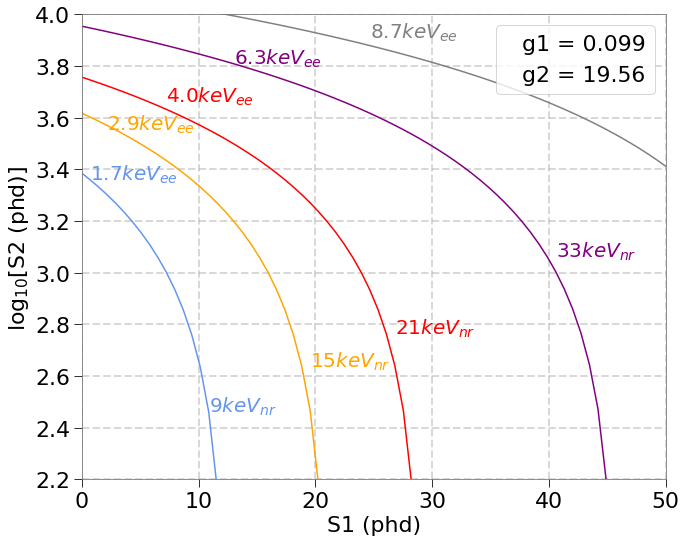
\includegraphics[width=\halffig]{figures/lxetpcs/E_contours.png}
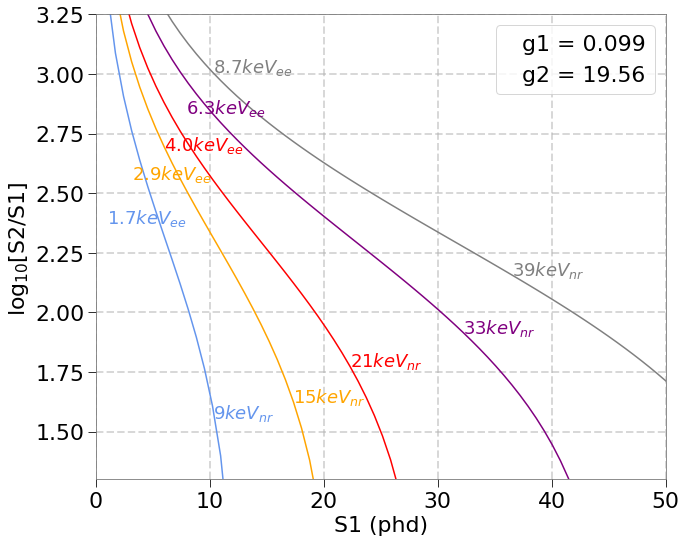
\includegraphics[width=\halffig]{figures/lxetpcs/E_contours2.png}
\caption{Plots showing combined energy contours in two common sets of axis units, for an example set of $g_{1}$ and $g_{2}$.}
\label{fig:e_contours}
\end{center}
\end{figure}


\section{Dual Phase Xenon TPCs for Dark Matter Detection}
Dual phase Xe \ac{TPC}s have been at the forefront of the hunt for dark matter in the last several decades. As described above, the xenon medium and detector technology make excellent low-background, rare-event searches with high signal yields. Dual phase Xe \ac{TPC}s also provide a few enhancements to \ac{WIMP} dark matter searches, but other dark matter or rare event searches are also possible with the same detector. This section describes the basic principle of \ac{WIMP} searches with \ac{LXe} \ac{TPC}s, then goes on to discuss how other types of dark matter searches are carried out with these detectors.


\subsection{WIMP Searches with LXe TPCs}
Dual-phase \ac{LXe} \ac{TPC}s are designed with \ac{WIMP} searches in mind. They have been very successful in reaching large areas of \ac{WIMP} parameter space. This section describes how \ac{WIMP} searches are carried out with this detector technology.

\subsubsection{ER, NR Discrimination}
\label{sec:er_nr_discrimination}
One of the most powerful features of \ac{LXe} \ac{TPC}s, which has made the technology especially useful in the hunt for \ac{WIMP} dark matter, is the ability to discriminate between electron recoils and nuclear recoils. \ac{WIMP} interactions are expected to be nuclear recoils, but most natural radioactivity ($\beta , \gamma$) are electron recoils. The amount of recombination for equal energy \ac{ER} and \ac{NR} is different, so for events with the same reconstructed energy $E$~(keV$_{ee}$), the ratio of S2/S1 is characteristically different. A useful discrimination space is log$_{10}$(S2/S1) vs S1, as the distributions of log$_{10}$(S2/S1) for \ac{ER} and \ac{NR} events of the same reconstructed energy are approximately Gaussian. Different calibration sources are used to develop a population of events known to be \ac{ER} and a population of events known to be \ac{NR}, these calibration sources reveal what is known as the \ac{ER} and \ac{NR} bands. Figure~\ref{fig:bands} shows the \ac{ER} and \ac{NR} bands from \ac{LUX}; the details of these calibrations are discussed further in Chapter~\ref{ch:lux}. 

\begin{figure}[htbp]
\begin{center}
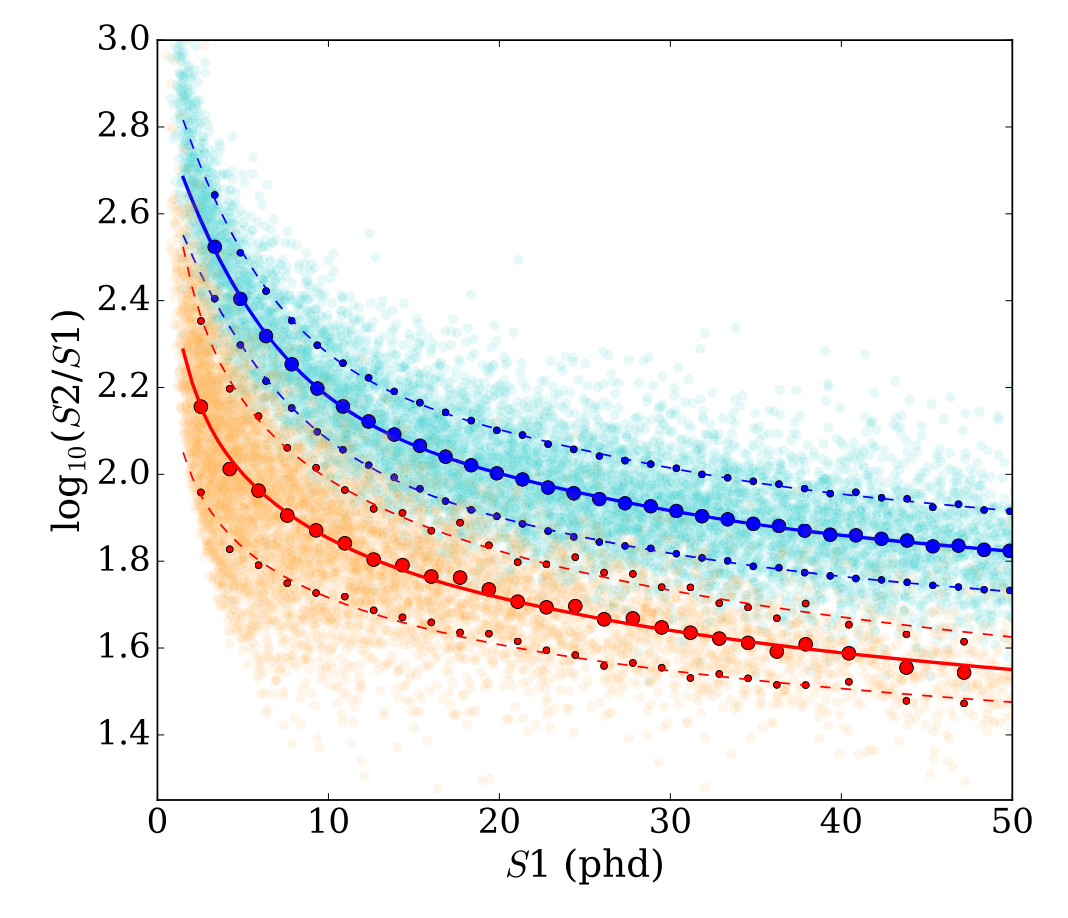
\includegraphics[width=0.65\textwidth]{figures/lxetpcs/bands.png}
\caption{Plot showing \acs{ER} and \acs{NR} bands from \acs{LUX}. Solid lines are the \acs{ER} and \acs{NR} Gaussian means, $\mu$; dotted lines are $\mu \pm 1 \sigma$. Figure from \cite{LUX:YieldsAndRecombination}. }
\label{fig:bands}
\end{center}
\end{figure}


In the course of a \ac{WIMP} search, the experimentalists are tasked with keeping a stable detector operating for months or years. In this time, the detector will see events of natural radioactivity and perhaps \ac{WIMP}s. The natural radioactivity appears in the \ac{ER} band (location of bands is known from calibration), and nuclear recoil events appear in the \ac{NR} band. Due to band overlap, only events appearing below the \ac{NR} mean are considered \ac{WIMP} candidates. This restriction cuts signal acceptance to 50\%, but allows dual-phase \ac{TPC}s to reject background electronic recoils at $\gtrsim$99\%. The background acceptance rate is known as \ac{ER} leakage. It is the fraction of events appearing below the \ac{NR} mean from the \ac{ER} calibration source. For a background rejection rate of 99.99\%, the \ac{ER} leakage is 0.01\%, this number determines the sensitivity of the detector.


\subsubsection{WIMP Rates and Cross Section}
\label{sec:wimp_rates}
The choice of direct detection for \ac{WIMP} searches was touched on in Section~\ref{sec:dm_detection_schemes}. Here, we go through the specifics of \ac{WIMP} rates and their cross section in \ac{LXe}. Although a multi-pronged approach including collider searches and indirect detection is ultimately necessary to understand dark matter, the \ac{LXe} \ac{TPC} technology profits from a few enhancements that make it especially suited for \ac{WIMP} searches. These enhancements are revealed below, as the \ac{WIMP} rates and cross section are outlined. 

\ac{WIMP}s scattering in the \ac{TPC} produce measurable nuclear recoils. The shape of this nuclear recoil spectrum eventually determines the number of \ac{WIMP} events observed, and it depends on both \ac{WIMP} properties and detector properties. The energy imparted to the nucleus depends on the \ac{WIMP} mass $M_{\chi}$ and velocity distribution, as well as the mass of the target nucleus $M_{T}$ and the cross section $\sigma$ that governs how effectively energy is transferred to the nucleus. Each of these pieces is described below, indicated with a \textbf{bold note} to aid the reader.

\textbf{Local Number Density and Velocity Distribution} Assuming a uniform, spherical dark matter halo, estimates for the local density of dark matter $\rho{\chi}$ can be made from astrophysical observations. The velocity distribution $f(v)$ is assumed to be isotropic and Maxwellian, with a cut-off at the escape velocity $v_{esc}$ of the Milky Way. If we account for the velocity of the Earth through the galactic plane $v_{E}$, the velocity distribution is shifted: $f(v) = f(v,v_{E})$. Following Lewin and Smith \cite{Lewin1996}, we can write the local number density:


\begin{equation}
\begin{split}
dn &= \frac{n_{0}}{k} f(v, v_{E}) d^{3}v \\
     &= \frac{n_{0}}{k} exp \Big( - \frac{(v + v_{E})^{2} }{ v_{0}^{2}} \Big) d^{3}v 
\end{split}
\end{equation}

Where $n_{0} = \rho_{\chi}/M_{\chi}$ is the average local number density of dark matter particles, $v_{0} \approx~230km/s$ \cite{Lewin1996} is the mean of the dark matter velocity distribution, and $k$ is a normalization constant such that $\int_{0}^{v_{esc}} dn \equiv n_{0}$. If the escape velocity is infinite, the normalization integral is easily evaluated:

\begin{equation}
k = \int_{0}^{2\pi} \int_{-1}^{1i} d(cos\theta)  \int_{0}^{\infty} f(v, v_{E}) v^{2}dv = (\pi v_{0}^{2})^{3/2} \equiv k_{0}
\end{equation}

$v_{esc}$ is not infinite ($v_{esc} \approx 544~km/s$ \cite{Baudis2014}), and so the normalization integral evaluates to:

\begin{equation}
k =  k_{0} \Big[ erf\big(\frac{v_{esc}}{v_{0}}\big) - \frac{2}{\pi^{1/2}} \frac{v_{esc}}{v_{0}} exp(- v_{exc}^{2} / v_{0}^{2} ) \Big]  \equiv k_{1}
\end{equation}

Although this is a more complicated expression, it should be noted the difference between $k_{0}$ and $k_{1}$ is less than \~0.5\%. 

\textbf{Scattering Rate} We now have a full picture of the local number density of dark matter, and we focus on the scattering rate in the detector. If we let $\sigma$ be the scattering cross-section per nucleus (the details of $\sigma$ are discussed later), the event rate per unit mass detector with target mass $M_{T}$ is:

%\begin{equation}
%\label{eq:rate}
%\begin{split}
%R &= \frac{N_{A}}{A} \sigma \int v~dn \\
%&= \frac{N_{A}}{A} \sigma n_{0} \langle v \rangle
%\end{split}
%\end{equation}

\begin{equation}
\label{eq:rate}
%\begin{split}
%dR &= \frac{N_{A}}{A} \sigma  v~dn \\
dR = \frac{1}{M_{T}} \sigma  v~dn 
%\end{split}
\end{equation}

%where $N_{A}$ is Avogadro's number. 
%It is useful to define $R_{0}$ for the test case $v_{E} = 0$ and $v_{esc} = \infty$:

%\begin{equation}
%R_{0} = \frac{\pi^{1/2}}{2} \frac{N_{0}}{A} \frac{\rho_{\chi}}{M_{\chi}} \sigma v_{0}
%\%end{equation}

%This allows us to re-write Equation~\ref{eq:rate} as:

%\begin{equation}
%\label{eq:integral_rate}
%\begin{split}
%R &= R_{0} \frac{\pi^{1/2}}{2} \frac{ \langle v \rangle }{v_{0}} \\
%   &=  R_{0} \frac{k_{0}}{k} \frac{1}{2\pi v_{0}^{4}} \int v f(v, v_{E}) d^{3}v
%\end{split}
%\end{equation}

%This is the differential rate per unit mass scattering in the target, but t
The experimentalist is concerned with the observable recoil energy spectrum produced by such a dark matter rate. A \ac{WIMP} of mass $M_{\chi}$ and initial energy $E_{\chi} = \frac{1}{2}M_{\chi}v^{2}$ scattering at angle $\theta$ (in the center-of-mass frame) will impart a recoil energy $E_{R}$ to a target nucleus of $M_{T}$

\begin{equation}
\label{eq:recoil}
E_{R} = r E_{\chi} \frac{1 - cos\theta}{2}
\end{equation}

Where $r$ is the kinematic factor:

\begin{equation}
r = \frac{ 4 M_{\chi}M_{T} }{ (M_{\chi} + M_{T})^{2}}
\end{equation}

Note that the kinematic factor indicates that recoil energies are greatest for $M_{\chi} \approx M_{T}$. \ac{SUSY} models favor \ac{WIMP} masses in the range 100GeV-1000GeV (Figure~\ref{fig:WIMPblobs}), which provides xenon ($M_{Xe} \approx$ 123 GeV) with an enhancement for \ac{WIMP}s when compared with other dark matter candidates. \ac{WIMP} scatters are assumed to be isotropic, so recoil energies are distributed uniformly in the range $0 < E_{R} < rE_{\chi}$ (i.e. Equation~\ref{eq:recoil} for $0 < cos\theta < 1$). We can put this together with Equation~\ref{eq:rate} to arrive at an differential rate per recoil energy in the detector -- i.e. the observable recoil spectrum for \ac{WIMP}-nucleus scattering. Note that equation Equation~\ref{eq:rate} is in terms of the \ac{WIMP} velocity $v$ and Equation~\ref{eq:recoil} is in terms of \ac{WIMP} energy $E_{\chi} = \frac{1}{2}M_{\chi}v^{2}$, so a change of variables is required. After the variable change, we can write:

\begin{equation}
\label{ref:dRdEr}
\frac{dR}{dE_{R}} =  \frac{\rho_{\chi}}{M_{\chi}} \frac{\sigma}{k} \Big( \frac{ M_{T} + M_{\chi}}{M_{T} M_{\chi}} \Big)^{2} \int_{v_{min}}^{v_{max}} \frac{1}{v} f(v,v_{E}) d^{3}v
\end{equation}

\textbf{WIMP-Xe Cross Section} Until now, we have left off discussion of the \ac{WIMP}-nucleus cross section $\sigma$. Equation~\ref{ref:dRdEr}, as it stands, is the \ac{WIMP} spectrum in the limit of billiard-ball coherent scattering. In reality, the nucleus has structure which must be accounted for; this is accomplished with a nuclear form factor $F = F(q)$. In addition, the cross-section is split into spin-independent ($\sigma_{SI}$) and spin-dependent ($\sigma_{SD}$) components:

\begin{equation}
\sigma = \sigma_{SI}F^{2}_{SI}(q) + \sigma_{SD}F^{2}_{SD}(q)
\end{equation}

The nuclear form factor, $F(q)_{SI, SD}$, decreases the cross section at higher momentum transfer; it is not discussed further. The two coherent terms $\sigma_{SI}$ and  $\sigma_{SD}$ are parametrized as follows:

\begin{equation}
\begin{split}
\sigma_{SI} &= \frac{4 \mu^{2} }{\pi} [ (A-Z) f_{n} + Zf_{p}]^{2} \\
 & \approx \frac{4 \mu^{2} A^{2}}{\pi} f_{n}^{2}
\end{split}
\end{equation}

Where $\mu$ is the usual reduced mass, and the second line takes into account that for \ac{SUSY} \ac{WIMP} models, the couplings to neutrons and protons are approximately equal ($f_{n} \approx f_{p}$).

\begin{equation}
\sigma_{SD} = \frac{32 G_{F} \mu^{2}}{\pi} \frac{J+1}{J} [\langle s_{n} \rangle a_{n} + \langle s_{p} \rangle a_{p}] ^{2}
\end{equation}

Where $G_{F}$ is the Fermi constant, $J$ is the total nuclear spin of the target, and $\langle s_{n,p} \rangle$ and $a_{n,p}$ represent values for neutron and proton spins and couplings, respectively. Note that $\sigma_{SI}$ scales as $A^{2}$, which indicates a larger cross-section for larger targets; this is the second enhancement from which xenon \ac{WIMP} detectors profit. $\sigma_{SD}$ lacks the $A^{2}$ scaling, and is smaller than $\sigma_{SI}$. This indicates that recoil-rates are dominated by spin-independent interactions. The two cases are treated separately, with collaborations releasing both spin-independent and spin-dependent \ac{WIMP} limits. In liquid xenon detectors, the odd-numbered nuclei $^{129}$Xe and $^{131}$Xe contribute to the spin-dependent rate. The enhancements for the \ac{WIMP} recoil rate in Xe, which come from the kinematic enhancement in rate and the $A^{2}$ cross section enhancement, are illustrated in Figure~\ref{fig:wimp_rates} \cite{Chepel2013}. For low-mass \ac{WIMP}s ($M_{\chi} \lesssim $ 10~GeV), xenon detectors quickly lose sensitivity when compared with cryogenic germanium and silicon detectors (Figure~\ref{fig:WIMPblobs}), and new analysis techniques are needed. 


\begin{figure}[htbp]
\begin{center}
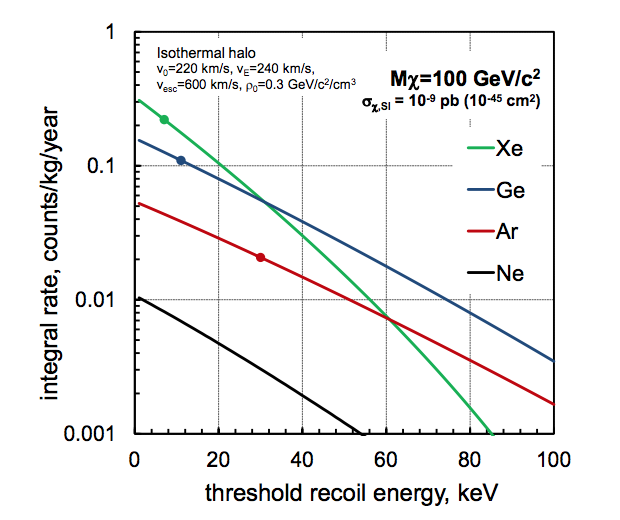
\includegraphics[width=0.8\textwidth]{figures/lxetpcs/wimp_rates.png}
\caption{Plot showing spin-independent \acs{WIMP} rates in common detector target materials, dots indicate typical thresholds for the targets. Xenon gains in favored \acs{SUSY} parameter space ($M_{\chi} \gtrsim$ 100~GeV) due to a kinematic enhancement ($M_{\chi} \sim M_{Xe}$ ) and a cross-section enhancement ($\sigma_{SI} \propto A^{2}$). Figure from \cite{Chepel2013}.}
\label{fig:wimp_rates}
\end{center}
\end{figure}

\begin{figure}[htbp]
\begin{center}
%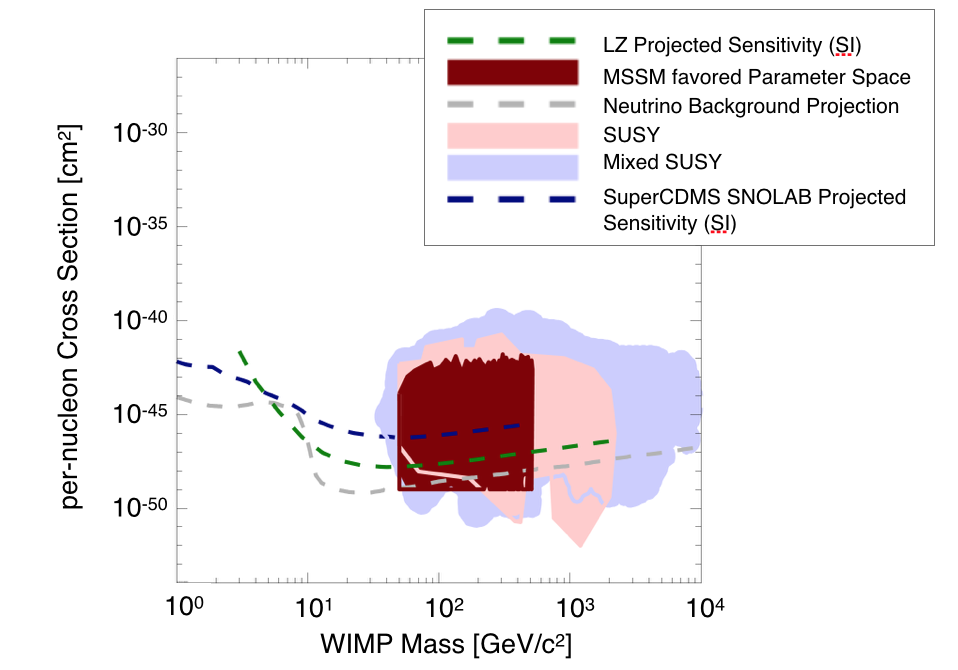
\includegraphics[width=0.9\textwidth]{figures/lxetpcs/WIMPblobs.png}
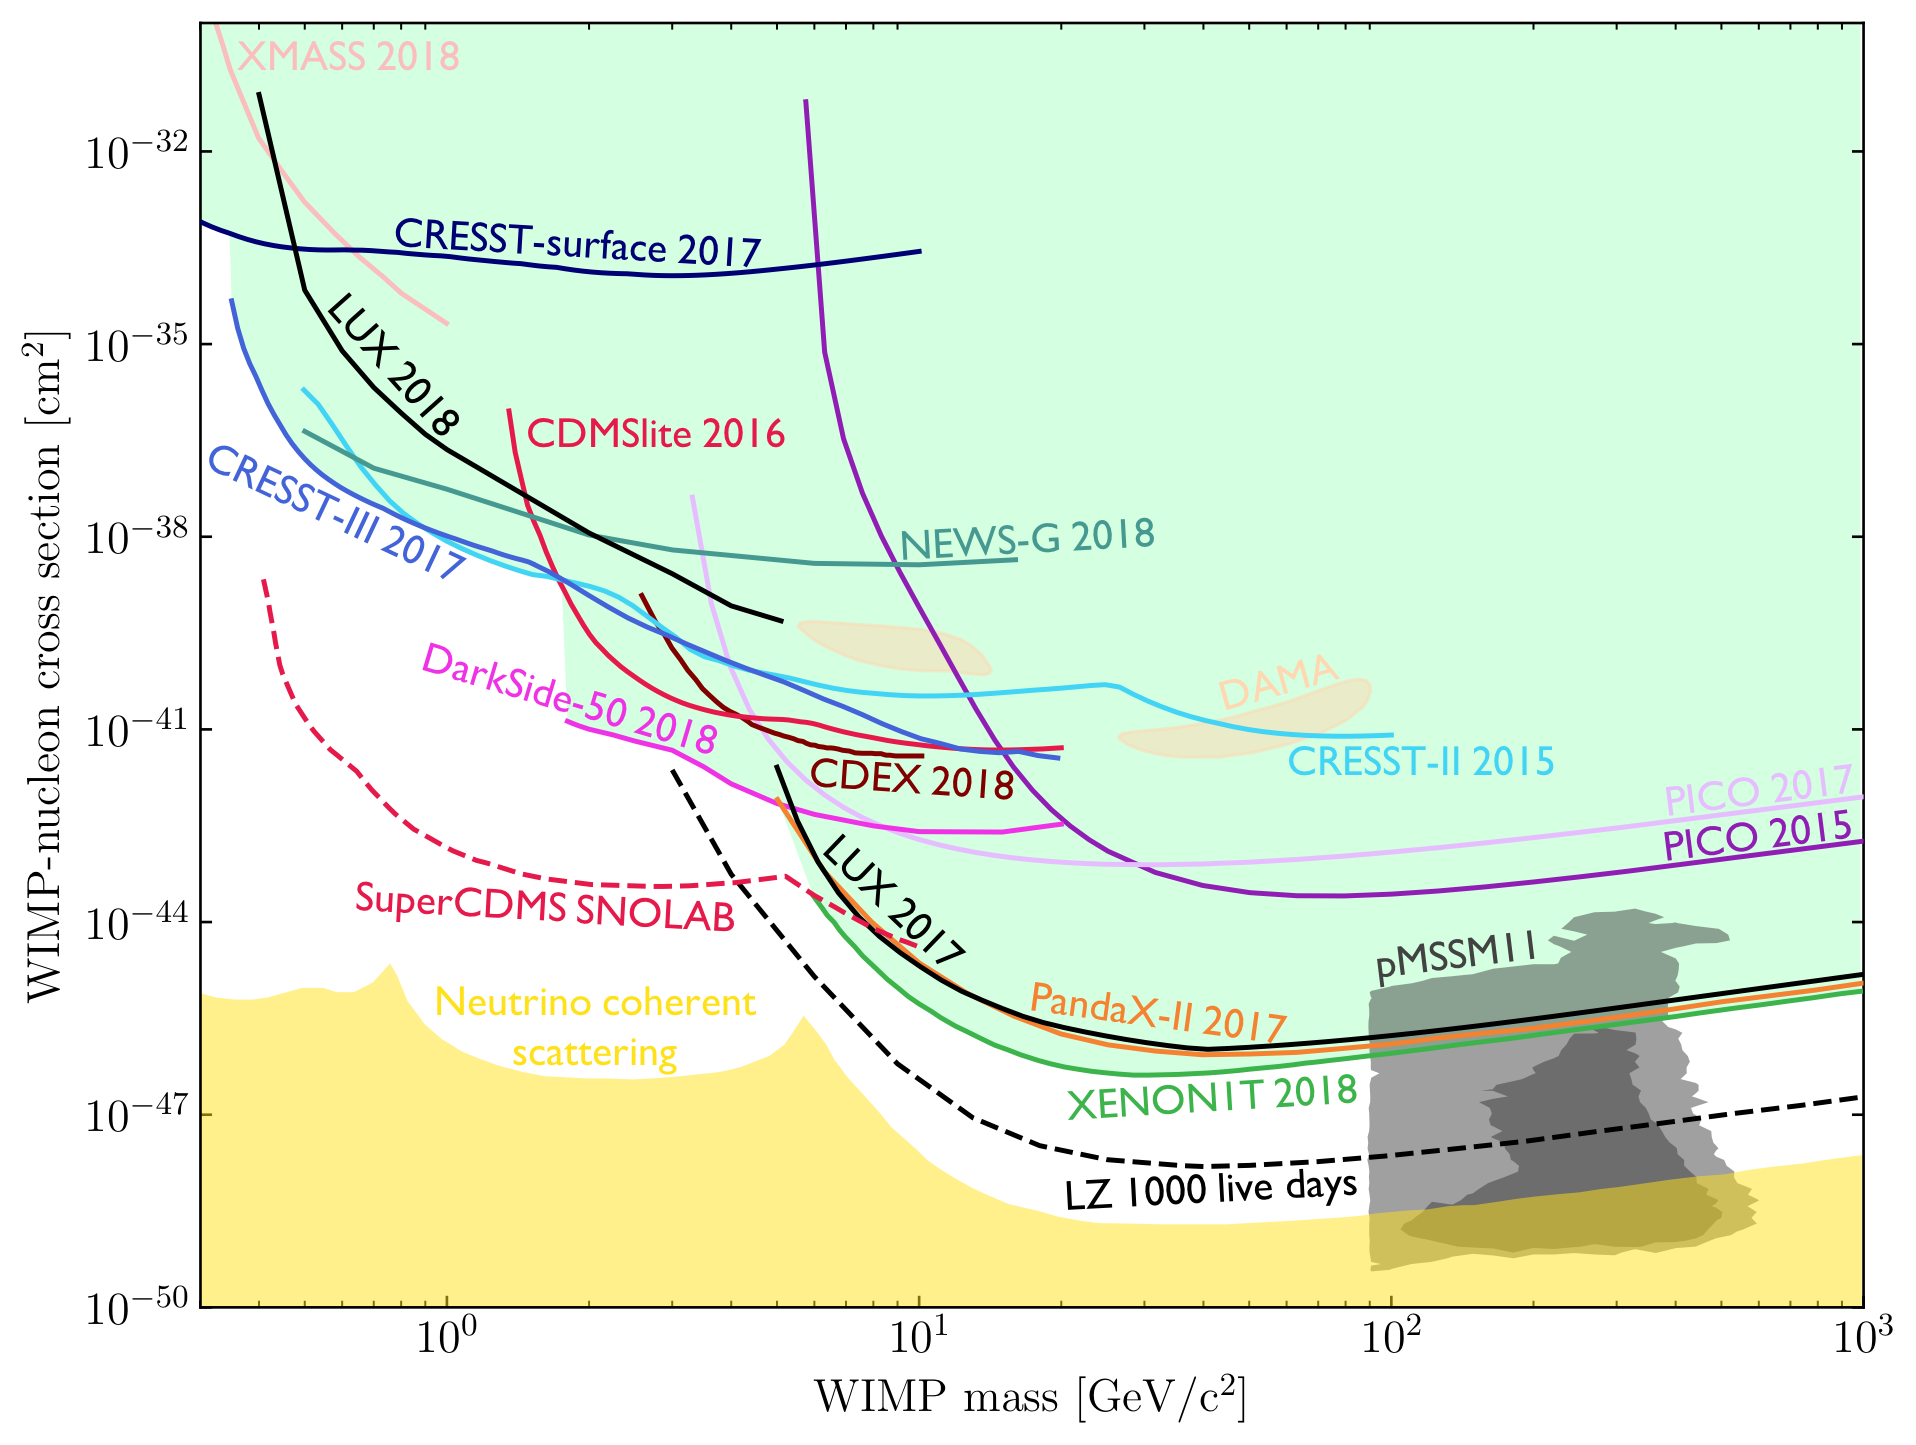
\includegraphics[width=\textwidth]{figures/lxetpcs/limits_all.png}
\caption{A summary of the excluded \acs{WIMP} parameter space by all experiments (green). Although next generation xenon experiments (LZ, black dashed) perform better for \acs{SUSY} \acs{WIMP} parameter space (gray region labelled pMSSM), germanium and silicon (SuperCDMS SNOLAB, pink dashed) can access other light dark matter parameter space below 10~GeV. The signal regions are from the DAMA collaboration, which has a long standing claim of detection with an annular modulation search; however, no other experiments have been able to reproduce such an observation. Plot courtesy of L. Tvrznikova, regenerated from \cite{snowmass}. }
\label{fig:WIMPblobs}
\end{center}
\end{figure}

%Projected limits of next-generation dark matter detectors and areas where \acs{SUSY} models predict the presence of \acs{WIMP}s. Although Xe (LZ, green dashed) performs better for \acs{WIMP} parameter space, Ge and Si (SuperCDMS, blue dashed) can access other light dark matter parameter space below 10~GeV. The plot was generated by http://dmtools.brown.edu/ 


\FloatBarrier
\subsection{Other Dark Matter Searches with LXe TPCs}
\label{sec:non_wimp_searches_with_lxetpcs}
The available \ac{SUSY} parameter space has dwindled greatly in the last few decades, due in large part to the success of this detector technology. Coupled with no observation of \ac{SUSY} at the \ac{LHC}, experimentalists are beginning to look to other models and parameter spaces for dark matter. New technologies are being developed and refined for new dark matter candidates, but already existing, well-understood detector technologies such as dual phase \ac{TPC}s can also be employed in the search for non-\ac{WIMP} dark matter. New analysis techniques can stretch the standard \ac{WIMP} analysis to lower masses, and to completely different dark matter candidates as well. This section briefly summarizes a few key analysis techniques that have been utilized by \ac{LXe} \ac{TPC}s to stretch the detector technology and access new parameter spaces. 

To understand how to expand a typical \ac{WIMP} analysis, we must first understand the thresholds that affect the current searches. Due to internal amplification of the S2 signal, \ac{LXe} \ac{TPC}s are capable of detecting events that produce a single electron. However, these detectors typically employ analysis thresholds much higher than their bare detection threshold for \ac{WIMP} searches. In their first \ac{WIMP} search results, the Xenon10 collaborationIn imposed an analysis threshold of 4.5~keV$_{nr}$ \cite{Xenon10WIMP}. The first \ac{LUX} results set an analysis threshold of 4.3~keV$_{nr}$ (with 2 < S1 (phd) < 30 and S2 (phd) > 200; S2 (electrons) $\gtrsim$ 8) \cite{LUXFirstResults}. The first Xenon100 results set an analysis threshold of 8.7~keV$_{nr}$ (4 < S1(phe) < 20 and S2 (phe) > 300; S2(electrons) $\gtrsim$ 10) \cite{Xenon100FirstResults}. Such thresholds are determined by the S1 light-collection efficiency of the detector; the analysis thresholds just described ensure the presence of an S1 in the event (S1 light collection efficiency is responsible for the steep rise in the xenon \ac{TPC} limits at low \ac{WIMP} mass). Without both an S1 and S2 in the event, the full ($x,y,z$) position cannot be re-constructed, and so a fiducial volume cut cannot be applied. Sorensen showed that the Xenon10 S2 pulse width carries a mild $z$-dependence \cite{Sorensen2010}, and so larger detectors with a long drift time may gain reliable $z$-position reconstruction via S2 pulse width \cite{SorensenS2Width}. Although no recent xenon \ac{TPC} has published such an analysis, the possibility exists for an ``S2-only'' search to access lower mass \ac{WIMP} parameter space. %allow dual-phase xenon \ac{TPC}s to reach lower \ac{WIMP} masses, and even other dark matter models. 

In 2011 the Xenon10 collaboration presented a search for low-mass (\~5 - 20 GeV) dark matter \cite{Angle2011}. They used both new analysis techniques and modified detector conditions for an S2-only search. The detector conditions were distinct from the Xenon10 \ac{WIMP} search in \cite{Xenon10WIMP}: the secondary scintillation gain was about 12\% higher, and the S2-sensitive trigger threshold was set at the level of a single electron. With this, the collaboration carried out a standard \ac{WIMP} analysis (i.e one based on the procedure presented in \ref{sec:wimp_rates}), with a lowered S2 analysis threshold of 4 electrons (1.4~keV$_{nr}$). Since Xenon10 is a small detector, they were not able to take advantage of S2-width z-correlations, but they employed a radial fiducial cut and other analysis techniques to produce the result in Figure~\ref{fig:xenon10lowmass}, which also shows the Xenon10 standard \ac{WIMP} analysis for comparison.The reason this analysis did not proceed down to the detection threshold of 1 electron is very interesting and has to do with a detector effect known as delayed electron noise or ``electron trains''; this phenomenon is discussed further in Chapter~\ref{ch:etrains}. 

\begin{figure}[htbp]
\begin{center}
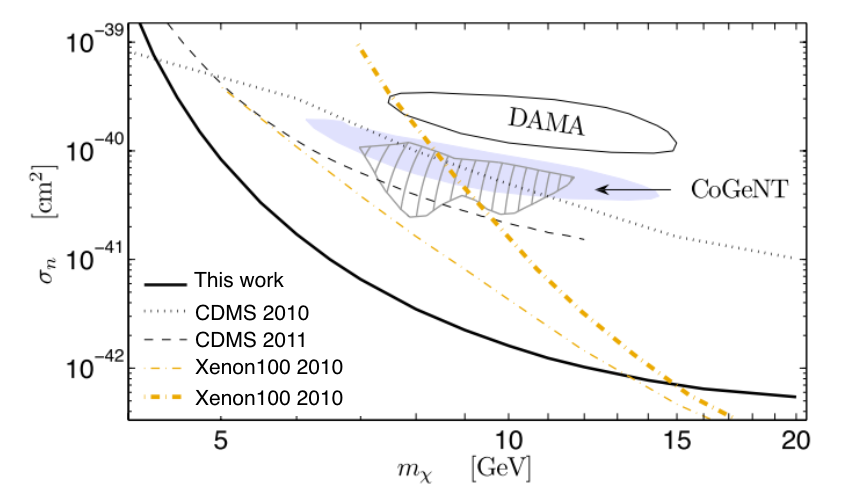
\includegraphics[width=0.65\textwidth]{figures/lxetpcs/xenon10lowmass.png}
\caption{Xenon10 low-mass \acs{WIMP} limit (black line) extended the range of the standard \acs{WIMP} result (yellow dashed lines). Figure from \cite{Angle2011}. }
\label{fig:xenon10lowmass}
\end{center}
\end{figure}


A few years later, Essig et al. used the information reported in \cite{Angle2011} and other Xenon10 publications to produce the first direct detection limits of sub-Gev dark matter \cite{Essig2012}. The detection threshold for \ac{WIMP}s in \ac{LXe} decreases sharply for $M_{WIMP} \lesssim 10~GeV$; however, this detection threshold is based on the assumption that the dark matter is interacting only with the xenon nucleus. If sub-GeV dark matter scatters with atomic \textit{electrons}, as opposed to nuclei, then it can produce observable signals of a few electrons. In \ac{LXe} \ac{TPC}s, the few electron signals are observable as S2s but the S1 signal is lost due to the difficultly of light collection for low energy events. The approach in the paper is to follow approximately the same procedure as in Section~\ref{sec:wimp_rates}, with a few but significant substitutions. The recoil energy ($E_{R}$ in Equation~\ref{eq:recoil}) must now account for the binding energy of the electron, and take a different form to refer to the recoil of the electron and not the nucleus. The cross section of interest is now $\sigma_{e}$, the sum over all of the differential ionization cross sections for electrons in the $(n, l)$-th shell. For a dark photon with mass $O$(MeV-GeV) coupled to the visible sector via kinetic mixing (a very generic class of standard model extensions discussed previously in Chapter~\ref{sec:dark_sector}), Essig et al. set the exclusion limit in the $m_{DM}-\sigma_{e}$ plane in Figure~\ref{fig:subGeV} (left). If there is some momentum-transfer enhancement due to e.g. scattering through an electric-dipole moment, $\sigma_{e} \longrightarrow \sigma_{e}F_{DM}(q) \equiv \bar{\sigma_{e}}$. Essig set exclusion limits for such dark matter candidates in Figure~\ref{fig:subGeV} (right).


\begin{figure}[htbp]
\begin{center}
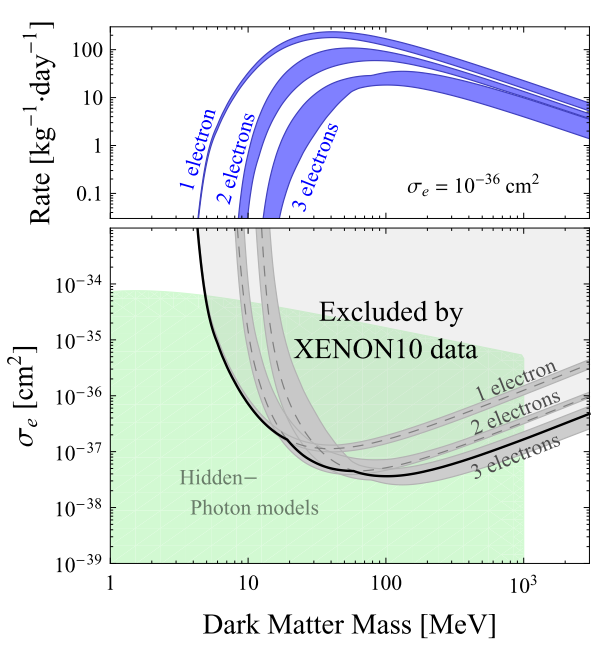
\includegraphics[width=\halffig]{figures/lxetpcs/subGeV.png}
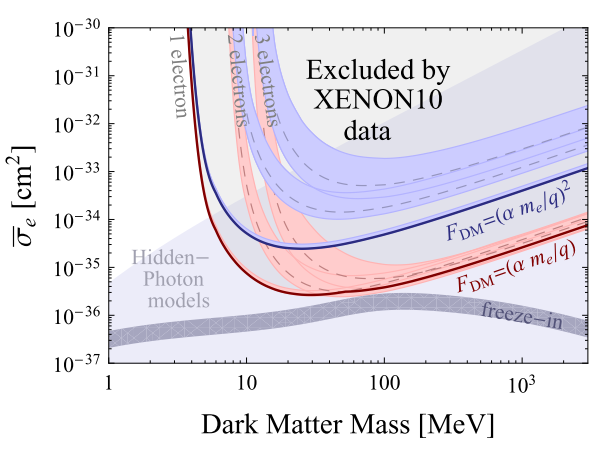
\includegraphics[width=\halffig]{figures/lxetpcs/subGeV2.png}
\caption{(left) Top: Expected 1,2,3-electron signal rates for Sub-GeV DM with $\sigma_{e} = 10^{-36}~cm^{2}$ and Bottom: exclusion limit set with Xenon10 few-electron signals. (right) Exclusion limits for dark matter scattering through an electric-dipole moment (red) and through a very light (<< keV) mediator (blue). Figures from~\cite{Essig2012}. }
\label{fig:subGeV}
\end{center}
\end{figure}


In addition to the dark sector, dual phase \ac{LXe} \ac{TPC}s can search for other dark matter signals from scattering on electrons. Annual modulation searches (in \ac{ER} or \ac{NR}) can provide clues to dark matter. Such searches take advantage of the fact that $v_{E}$ varies with the rotation of the earth around the sun, reaching a maximum in June and minimum in December. The modulation in $v_{E}$ leads to a modulation in the recoil rate observed in the detector. Searches for dark matter-induced rate modulations can offer a generic approach to identify dark matter interactions, complementary to the model-driven dark matter searches. The \ac{LUX} experiment carried out such a search, looking at \ac{ER} modulations in an energy rage of interest (2-6~keV$_{ee}$). This energy range was chosen to overlap with the DAMA/LIBRA Collaboration's long-standing and controversial claim of dark matter modulation on a target of NaI(Tl), which appears strongest around a recoil energy of 3~keV$_{ee}$ (their signal region is shown in Figure~\ref{fig:WIMPblobs}). \ac{LUX} found no significant indication of rate modulation \cite{LUXModulation}. If future large dual phase \ac{TPC}s like XenonNT and LZ observe an \ac{NR} \ac{WIMP} signal, the additional positive identification of a modulation signal of the \ac{NR} signal would be a smoking-gun for \ac{WIMP} discovery. 

Another dark matter candidate that could produce an electron recoil signal in xenon is the axion (or more generally, axion-like-particles). For searches such as these, a signal model is produced from the spectrum of axions from different sources, such as galactic axions or solar axions. The resulting signal model is an \ac{ER} spectrum that accounts for finite detector energy resolution and threshold. The signal model spectrum is compared to the observed \ac{ER} spectrum in the appropriate energy ranges, resulting in a confidence statement mass of the axion $m_{A}$ and the axio-electric coupling $g_{Ae}$. The results of searches for solar axion and galactic axion signals are shown in Figure~\ref{fig:axions}.

\begin{figure}[htbp]
\begin{center}
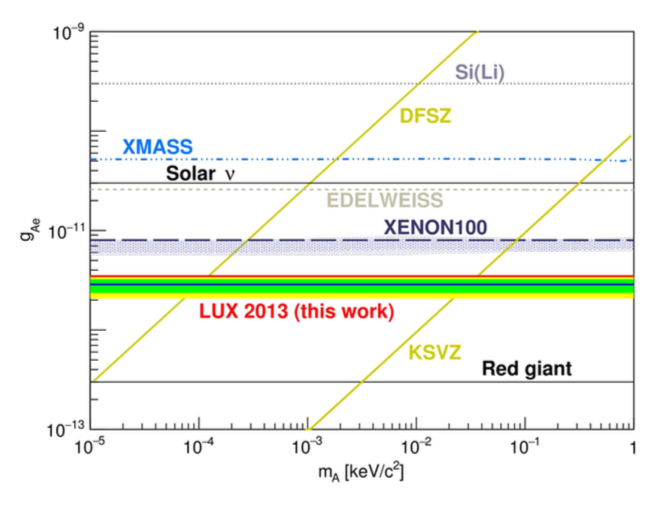
\includegraphics[width=\halffig]{figures/lxetpcs/axions1.png}
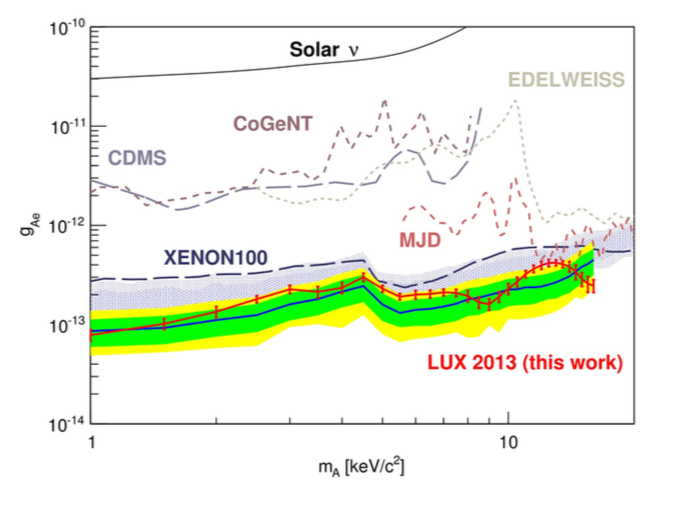
\includegraphics[width=\halffig]{figures/lxetpcs/axions2.png}
\caption{(left) Recent limits on solar axion coupling and mass (right) recent limits on galactic axion coupling and mass. Figure taken from \cite{LUXAxions}. }
\label{fig:axions}
\end{center}
\end{figure}

Finally, a model-independent search for \ac{LIP}s is possible in dual phase xenon \ac{TPC}s. As discussed in Chapter~\ref{sec:dark_sector}, \ac{LIP}s appear in dark sector models with a masses dark photon, where another dark sector particle couples to the standard model electron via kinetic mixing of the dark photon and standard model photon. \ac{LIP}s deposit energies that can be described with particles of effective fractional charge. Chapter~\ref{ch:lips} describes the signal model and analysis method to search for \ac{LIP}s in \ac{LUX}. 





%*****************************************
%*****************************************
%*****************************************
%*****************************************
%*****************************************

